\chapter{Marco Teórico}

% En este capítulo, se presenta las principales tecnologías de detección en primer  plano del objeto en movimiento, descripción y extracción de características,  clasificación y reconocimiento del movimiento humano. Basado en el flujo óptico para la detección de objetos en movimiento. Como también la imagen de flujo de energía óptico para la detección de características de movimiento y se adoptaron redes neuronales convolucionales de región para elegir  características y reducir la dimensión. Luego, gracias al clasificador de máquina de vectores de soporte que puede ser entrenado y utilizado para clasificar y reconocer acciones; es posible distinguir efectivamente las acciones humanas y mejorar significativamente la precision del reconocimineto de las acciones humanas.

\section{Sistema de video vigilancia}
La videovigilancia consiste en el despliegue de cámaras de vídeo que funcionan como video-filmadoras, las cuales guardan el contenido recolectado en un almacén digital el cual puede ser visto en un monitor central. Un sistema de video-vigilancia consiste en una instalación de seguridad cuya finalidad es el control y supervisión visual en tiempo real de instalaciones locales y remotas, mediante el uso de múltiples cámaras de vigilancia, así como de sistemas de visualización, grabación y archivo. Estos sistemas ayudan a proteger a las personas, bienes y recursos, mantienen una alerta activa y poseen un gran efecto disuasorio \cite{wikipedia:vvigilancia}.\\

El sistema captura imágenes y vídeos, que pueden ser comprimidos, almacenados, o enviados por una red de comunicación y pueden ser instalados en cualquier ambiente. En la figura \ref{fig:sistema_video_vigilancia} se visualiza el conjunto de elementos que forman un sistema de video vigilancia. Este sistema compone de un conjunto de cámaras que estan conectados directamente a un grabador de video en red o N.V.R. o por sus siglas en inglés(Network Video Recorder), el cual permite la visualización de lo que las cámaras captan en un monitor local y por medio de una conección a un punto de acceso a internet, permite la visualización de esta transmisión en dispositivos externos a la red local.\\

\begin{figure}[H]
    \begin{center}
        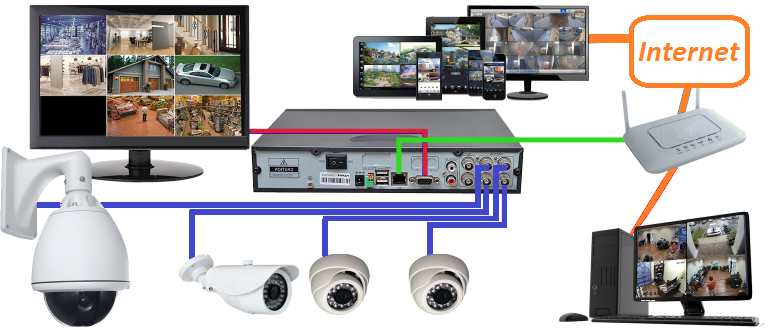
\includegraphics[width=9cm]{img/capitulo_2/sis_videovigilancia.png}
    \end{center}
    \caption{Sistema actual de videovigilancia\\Fuente: Web}
    \label{fig:sistema_video_vigilancia}
\end{figure}

La creciente demanda en el mercado de la vigilancia ha reducido costos en este tipo de sistemas, lo cual permitió que desarrolladores y fabricantes diseñen nuevas implementaciones de sistemas de video vigilancia agregándoles diversas capacidades dependiendo de la tecnología utilizada en su desarrollo. En la figura \ref{fig:surveillance-market} se muestra como el mercado global de la video vigilancia fue avaluado en 42.9 billones de dólares en 2019 y esta proyectado alcanzar a los 69.1 billones de dólares hasta el 2026, registrando una taza de crecimiento anual compuesta del 10\% desde el 2020 al 2026. \cite{marketsandmarkets:market-surveillance}\\

\begin{figure}[H]
    \begin{center}
        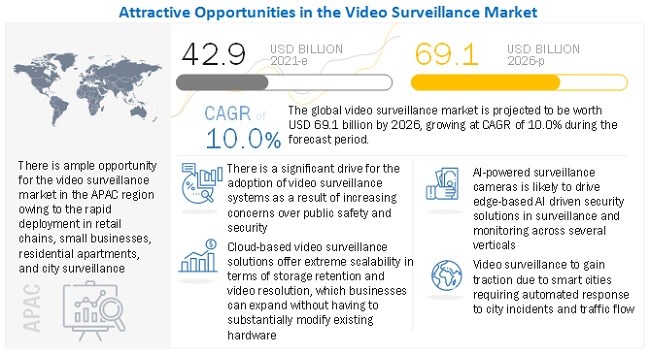
\includegraphics[width=13cm]{img/capitulo_2/surveillance-market.jpg}
    \end{center}
    \caption{Proyección del mercado de la video-vigilancia\\Fuente: MarketsAndMarkets(web)}
    \label{fig:surveillance-market}
\end{figure}

El aspecto más importante a resaltar en el mercado de la video-vigilancia es la potenciación de funcionalidades de estos sistemas gracias a la Inteligencia Artificial (I.A.) y la escalabilidad por servicios basados en la nube. Las ramas de inteligencia artificial como el Machine Learning(Aprendizaje Automático) y el Deep Learning(Aprendizaje profundo) permitiran potenciar las capacidades de este tipo de sistemas.

Para el desarrollo del prototipo propuesto se implementan todos los componentes involucrados en el sistema de video-vigilancia como ser:
\begin{itemize}
    \item Cámaras (denominados "nodos")
    \item Servidor TCP (Protocolo de transmisión para sockets de conección)
    \item Servidor HTTP (Protocolo web para la transmisión en vivo de video)
    \item Módulo SMTP (Módulo de comunicación para correo electrónico para notificaciones)
\end{itemize}

Para la implementación del prototipo es necesario describir los conceptos necesarios para la captura de fotogramas de video, transmisión de paquetes por un enlace tcp/ip, reconstrucción de mensajes, consolidación y procesamiento de imagenes, y transmisión de video en vivo. A continuación se detallan los conceptos teóricos y prácticos descritos anteriormente que son relevantes en el desarrollo del prototipo de sistema de video-vigilancia propuesto.\\

\section{Inteligencia Artificial}
La Inteligencia Artificial (I.A.), es una tecnología innovadora que en los últimos tiempos no esta reservado solo para la investigación si no más bien ha ido formando parte en el desarrollo de la sociedad. El cerebro es el órgano más increible del cuerpo humano; establece la forma en la que percibimos las imágenes, sonido, olores, sabores y el tacto; por lo tanto permite al ser humano almacenar recuerdos, experimentar emociones e incluso soñar. Sin él, el ser humano sería un organismo primitivo, incapaz de otra cosa que el más simple de los reflejos. Por lo tanto el cerebro es lo que hace a este ser, un ser inteligente.\\

Durante décadas se ha investigado para construir máquinas inteligentes con cerebros como el del ser humano; asistentes robotizados para limpiar los hogares, coches que se conducen por solos, microscopios que detecten enfermedades automáticamente. Pero en la construcción de estas máquinas artificialmente inteligentes se presentan problemas computacionales complejos; problemas que el cerebro humano puede resolver en una fracción de segundos. Las formas de analizar y resolver este tipo de problemas, es el campo de estudio de la Inteligencia Artificial.

\begin{figure}[H]
    \begin{center}
        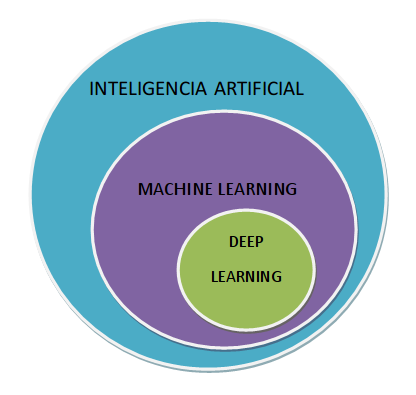
\includegraphics[width=8cm]{img/capitulo_2/ia.png}
    \end{center}
    \caption{Campo de acción de la Inteligencia Artificial.\\Fuente: Web}
    \label{fig:ia}
\end{figure}

A menudo los términos Inteligencia Artificial, Aprendizaje Automático (Machine Learning) y Aprendiazaje Profundo (Deep Learning) son usados de manera indistinta, pero se debe tener en cuenta su significado diferente. Por los años `80 la Inteligencia Artificial era una característica que se alcanzaba al definir un conjunto de reglas que decían que hacer en un determinado momento, de esta manera un sistema `inteligente' solo obedecía reglas de acción programadas \cite{researchgate:ia}. En la figura \ref{fig:ia} se ilustra como la Inteligencia Artificial engloba a sus subcampos de estudio como ser el Machine Learning y el Deep Learning.

\section{Machine Learning (Aprendizaje de Máquina)}
Es un subcampo de la Inteligencia Artificial cuyo objetivo es entender la estructura de la información y ajustar estos datos en modelos que puedan ser entendidos y utilizados por las personas. \cite{digitalocean:machinelearning}.\\

A diferencia de la computación tradicional, donde los algoritmos resuelven problemas específicos, los algoritmos de Machine Learning entrenan a las computadoras con datos de entrada y emplean análisis estadístico para generar valores de salida que se clasifican según a un rango específico. Por eso el Machine Learning facilita a las computadoras construir modelos a partir de datos ejemplo para automatizar el proceso de toma de decisiones basados en estos datos.\\

\begin{figure}[H]
    \begin{center}
        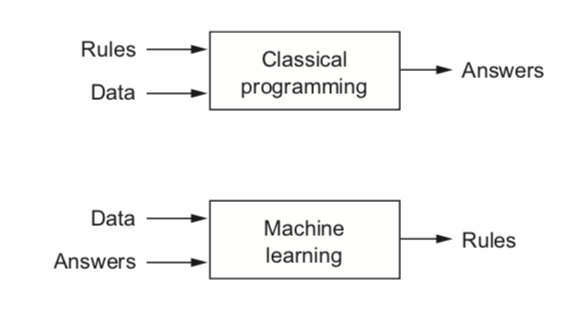
\includegraphics[width=10cm]{img/capitulo_2/machinelearning.png}
    \end{center}
    \caption{Diferencias entre programación clásica y M.L.\\Fuente: Deep Learning with Python}
    \label{fig:classical_ml}
\end{figure}

En la figura \ref{fig:classical_ml} se aprecia la diferencia y similitud entre la programación clásica de la inteligencia artificial de los años `80 y las novedosas técnicas del aprendizaje automático. La programación clásica necesita de reglas y datos de entrada para que esta funcione como un sistema inteligente y pueda dar una respuesta, mientras que el Machine Learning necesita de datos y sus respectivas respuestas esperadas, para identificar patrones que los relacionen; y de esta manera permitiendo desarrollar reglas que generarán respuestas para nuevos datos.

\subsection{Métodos de Machine Learning}
En el Machine Learning, las tareas son generalmente clasificadas en grandes categorias, las cuales estan basadas en el modo en el que el ``aprendizaje'' es ejecutado.\\

Los métodos más adoptados en el Machine Learning son: el aprendizaje supervisado, que entrena un algoritmo basado en un ejemplo de entrada y salida el cual esta categorizado por un humano, y el aprendizaje no supervisado, que proporciona el algoritmo sin ningún dato categorizado permitiendo encontrar una estructura dentro de los datos de entrada.\

\subsubsection{Aprendizaje Supervisado}
La computadora esta provista con entradas de ejemplo las cuales están categorizadas con sus respectivas salidas esperadas. El propósito de este metodo consiste en que el algoritmo pueda 1 ``aprender'' comparando la actual salida con las salidas esperadas para encontrar errores y en consecuencia modificar el modelo. El aprendizaje supervisado por lo tanto usa patrones para predecir valores categorizados en datos no categorizados.\

\subsubsection{Aprendizaje No Supervisado}
La información provista a la computadora no está categorizada, por lo que los algoritmos de aprendizaje buscan similitudes entre los datos de entrada. Como los datos no etiquetados son más abundantes que los datos etiquetados, los métodos de aprendizaje automático que facilitan el ``aprendizaje'' pasan a ser más importantes.\

\section{Deep Learning (Aprendizaje profundo)}
Según la figura \ref{fig:ia}, el aprendizaje profundo es un subcampo dentro del Machine Learning, el cual hace uso de distintas redes neuronales para lograr el ``aprendizaje'' de sucesivas capas de representación que son relevantes para los datos.\\

El término Deep ``profundo'', hace referencia a la cantidad de capas de representación que se utilizan en un modelo; en general es posible utilizar decenas incluso cientos capas de representación, los cuales aprenden de forma automática a medida que el modelo es entrenado con los datos \cite{iaarbook:artificialvision}.

\subsection{Redes Neuronales}
Las redes neuronales artificiales son un modelo inspirado en el funcionamiento del cerebro humano. Está formado por un conjunto de nodos conocidos como neuronas artificiales que están conectadas y transmiten señales entre sí. Estas señales se transmiten desde la entrada hasta generar una salida. En la figura \ref{fig:classical_ml} se aprecia la estructura propia de una neurona artificial.\\

\begin{figure}[H]
    \begin{center}
        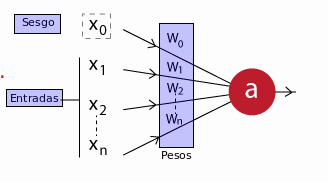
\includegraphics[width=7cm]{img/capitulo_2/neurona.png}
    \end{center}
    \caption{Ilustración de una Neurona artificial
        \\Fuente: Web}
    \label{fig:classical_ml}
\end{figure}

El objetivo principal de un modelo neuronal, es aprender modificándose automáticamente a si mismo, llegando a realizar tareas complejas que no podrían ser realizadas mediante la clásica programación basada en reglas. De esta forma se pueden automatizar funciones que al principio solo podrían ser realizadas por personas. Con su semejanza al del cerebro humano, las redes reciben una serie de valores de entrada y cada una de estas entradas llega a un nodo llamado neurona.\\

Las neuronas de la red están a su vez agrupadas en capas que forman la red neuronal. Cada una de las neuronas de la red posee a su vez un peso, un valor numérico, con el que modifica la entrada recibida. Los nuevos valores obtenidos salen de las neuronas y continúan su camino por la red. Este funcionamiento puede observarse de forma esquemática en la figura \ref{fig:estructura_red_neuronal}.\\

\begin{figure}[H]
    \begin{center}
        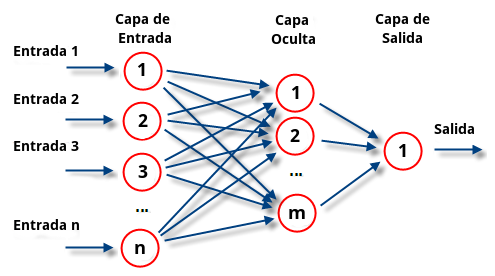
\includegraphics[width=7cm]{img/capitulo_2/Redes_neuronales_esquema.png}
    \end{center}
    \caption{Ilustración de una Red Neuronal
        \\Fuente: Web}
    \label{fig:estructura_red_neuronal}
\end{figure}

Una vez que se alcanza el final de la red se obtiene una salida que será la predicción calculada por la red. Cuantas más capas posea la red y más compleja sea, también serán mas complejas las funciones que pueda realizar. Para conseguir que una red neuronal realice las funciones deseadas, es necesario \textbf{entrenarla}.\\

El entrenamiento de una red neuronal se realiza modificando los pesos de sus neuronas para que consiga extraer los resultados deseados. Para ello lo que se hace es introducir datos de entrenamiento en la red, en función del resultado que se obtenga, se modifican los pesos de las neuronas según el error obtenido y en función de cuanto haya contribuido cada neurona a dicho resultado. Este método es conocido como Backpropagation o propagación hacia atrás. Con este método se consigue que la red aprenda, consiguiendo un modelo capaz de obtener resultados muy acertados incluso con datos muy diferentes a los que han sido utilizados durante su entrenamiento \cite{atriainnovation:ia}.\\

Estas redes neuronales son utilizadas para tareas de predicción y clasificación. Esta técnica se ha convertido en una pieza clave para el desarrollo de la Inteligencia Artificial, como se describió previamente es uno de los principales campos de investigación y el que más esta evolucionando con el tiempo, ofreciendo cada vez soluciones más complejas y eficientes.

\subsubsection{Redes neuronales convolucionales}
Dentro del conjunto de tipos de redes neuronales tenemos las convolucionales, que específicamente serviran en el campo de la visión artificial. Las redes neuronales convolucionales son un algoritmo de Aprendizaje Profundo (Deep Learning) que está diseñado para trabajar con imágenes, tomando estas como entrada, asignándoles importancias (pesos) a ciertos elementos en la imagen para así poder diferenciar unos de otros.\\

\begin{figure}[H]
    \begin{center}
        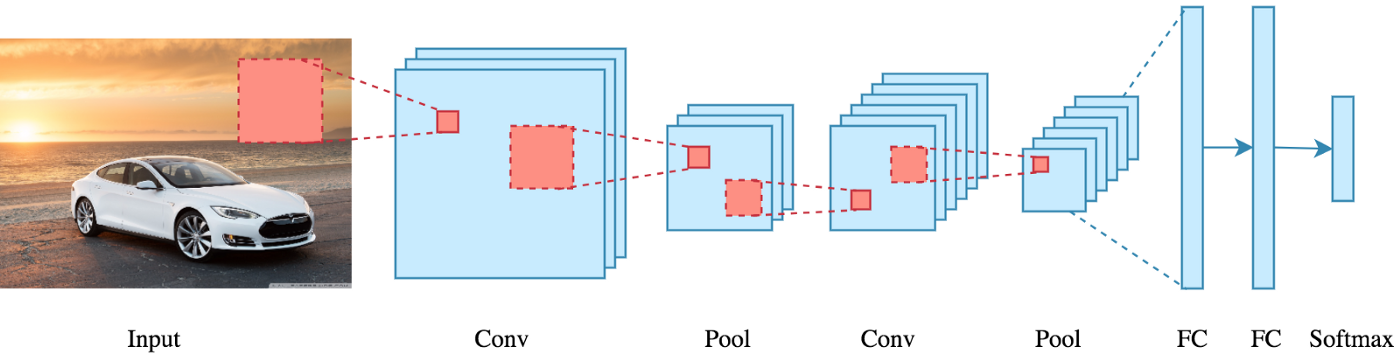
\includegraphics[width=10cm]{img/capitulo_2/convolucional.png}
    \end{center}
    \caption{Ilustración de una Red Neuronal Convolucional
        \\Fuente: Web}
    \label{fig:red_neuronal_convolucional}
\end{figure}

Este es uno de los principales algoritmos que ha contribuido en el desarrollo y perfeccionamiento del campo de visión por computadora. Las redes convolucionales contienen varias capas ocultas como se ilustra en la figura \ref{fig:estructura_red_neuronal}, donde las primeras puedan detectar líneas, curvas y así se van especializando hasta poder reconocer formas complejas como un rostro, siluetas, etc. \cite{convolutional:ia}. \\

\begin{figure}[H]
    \begin{center}
        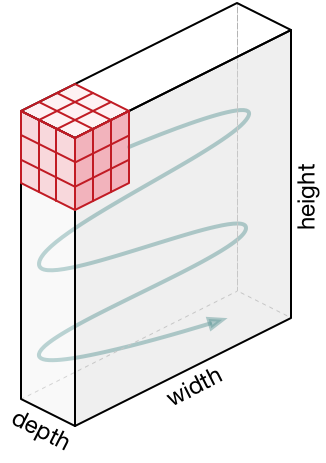
\includegraphics[width=3cm]{img/capitulo_2/kernel.png}
    \end{center}
    \caption{Movimiento del Kernel
        \\Fuente: Web}
    \label{fig:kernel}
\end{figure}

El proceso que se distingue de estas redes son las convoluciones. El cual consiste en tomar un grupo de píxeles de la imagen de entrada e ir realizando un producto escalar con un kernel. El kernel recorrerá todas las neuronas de entrada y obtendremos una nueva matriz, la cual será una de las capas ocultas. En el caso de que la imagen sea de color se tendrán 3 kernels del mismo tamaño que se sumarán para obtener una imagen de salida.\\

El kernel en las redes convolucionales se considera como un filtro que se aplica para extraer ciertas características importantes o patrones de esta y es usado para detectar bordes, enfoque, desenfoques, entre otras características de la imagen y es logrado para la convolución entre la imagen y el kernel.

Este proceso se desarrolla entre la imagen y el kernel, con la finalidad de que este filtro o kernel recorra toda la imagen (pixel por pixel). Por lo general, el kernel es de menor tamaño que la imagen. La convolución permite multiplicar el kernel con la porción de imagen escogida, realiza un producto escalar a medida que el kernel se va desplazando; por esta razón es un proceso iterativo .\\

Es una operación que se usa en las redes convolucionales. El padding se aplica agregando píxeles de valor cero alrededor de la imagen original.
Tiene dos usos:
El primero es para que al realizar la convolución la imagen resultante sea de igual tamaño que la imagen original.
El segundo es cuando se tiene información relevante en las esquinas de la imagen por lo que al realizar convolución el filtro pasa más por el centro de la imagen que en las esquinas, por lo que se aplica el padding para tener la información más relevante cerca del centro.\\

Las tareas comunes de este tipo de redes son: detección o categorización de objetos, clasificación de escenas y clasificación de imágenes en general. La red toma como entrada los pixeles de una imagen. 


\section{Visión por Computadora}
La visión por computadora es una técnica de recolección de información que surge por la inspiración en el sistema visual humano, el cual es la principal fuente de información para el cerebro. Su meta es de modelar y automatizar el proceso de reconocimiento visual de objetos en la vida real.\\

De los cinco sentidos que poseen las personas, la vista es la más importante. Por lo tanto la visión, es una tarea de procesamiento de información; pero tiene un grado de complejidad elevado, ya que para saber que es lo qué hay en el mundo nuestros cerebros deben ser capaces de representar esta información en toda su abundancia de color, forma, movimiento, detalle y belleza. \cite{iaarbook:artificialvision}\\

Por lo tanto, la visión por computadora o visión artificial compone de un conjunto de herramientas y métodos que permiten obtener, procesar y analizar imágenes del mundo real, con el objetivo de ser tratadas por una computadora. Estos métodos van a permitir automatizar un amplio conjunto de tareas al aportar a las computadoras información que es necesaria para la toma de desiciones en sus tareas asignadas. La visión por computadora trata de imitar a la visión humana, usando geometría y un enfoque estadístico para tratar el problema.\\

\subsection{Aplicaciones}
Esta rama de la Inteligencia Artificial aún sigue en investigación y mejoras donde sus aplicaciones más comunes son:

\begin{itemize}
    \item \textbf{Reconocimiento óptico de caracteres:} Detección automática de símbolos que pertenecen a un alfabeto.
    \item \textbf{Inspección robotizada:} Revisión rápida de piezas para garantizar la calidad de componentes fabricados.
    \item \textbf{Modelado 3D:} Construcción de modelos 3D a partir de fotografías.
    \item \textbf{Imágenes médicas:} Análisis de radiografías.
    \item \textbf{Conducción segura:} Detección de obstáculos por medio de un sistema de conducción asistida por cámaras.
    \item \textbf{Vigilancia:} Monitoreo de intrusos, análisis del tráfico vial, monitoreo de piscinas, etc.
    \item \textbf{Detección de rostros:} Mediante algoritmos de reconocimiento facial se reconocen rostros usados en métodos de biometría.
\end{itemize}

\subsection{OpenCV}
Es una biblioteca de uso libre para el desarrollo de aplicaciones usando visión artificial desarrollada por Intel. Esta libreria reune diversas caracteristicas que la hacen popular, por ejemplo: 
\begin{itemize}
    \item Permite su uso para fines comerciales y de investigación.
    \item Se encuentra disponible par varias plataformas como ser GNU/Linux, Mac OS, Windows y Android.
    \item Documentación completa y explicada, con una comunidad de desarrolladores activa.
\end{itemize}

\begin{figure}[H]
    \begin{center}
        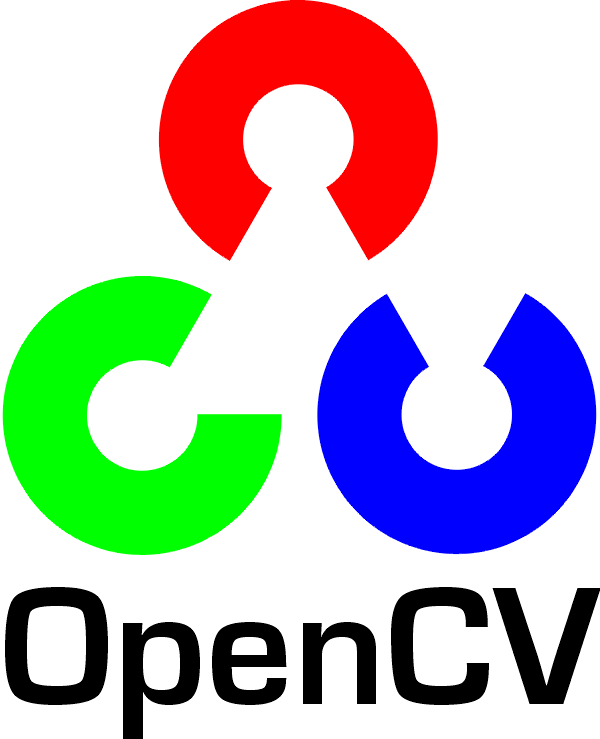
\includegraphics[width=3cm]{img/capitulo_2/cv2_logo.png}
    \end{center}
    \caption{Logotipo de la libreria\\Fuente: Web}
    \label{fig:cv2_logo}
\end{figure}

Esta biblioteca permite:
\begin{itemize}
    \item El procesamiento de imágenes en su escalado, eliminación de ruido y formateo de imagen y video.
    \item El uso y modificación de sus 2500 modelos pre-optimizados que son incluidos en la libreria, acorde a las necesidades del usuario.
    \item El uso del estado del arte de modelos de visión por computadora como también de aprendizaje de máquina (Machine Learning).
    \item El desarrollo de modelos en varias categorías de investigación como ser: reconocimiento facial, detección y seguimiento de objetos, extracción de modelos 3D, etc.
\end{itemize}

Una de las características mas interesantes de OpenCV es el reconocimiento facial. OpenCV, en su extensa biblioteca de funciones, brinda las capacidades para realizar las tareas de preprocesamiento sin ningún problema, así como los algoritmos de predicción. Además de usar el algoritmo de detección de objetos, es posible usar el seguimiento de objetos, para identificar rostros en una transmisión de video. OpenCV incluso posee funciones para configurar fácilmente el modelo en una transmisión en vivo, como en un video pregrabado \cite{medium:opencv}. 

% \section{Redes Neuronales}

\section{Protocolos de red}
Un protocolo es un método estándar que permite la comunicación entre procesos (que potencialmente se ejecutan en diferentes equipos) y un conjunto de reglas y procedimientos que deben respetarse para el envío y la recepción de datos a través de una red.

\subsection{TCP/IP}
El Protocolo de Control de Transmisión es uno de los protocolos fundamentales en Internet. Fue creado entre los años 1973-1974 por Vint Cerf y Robert Kahn. Este es uno delos principales protocolos de la capa de transporte del modelo TCP/IP. En el nivel de aplicación, posibilita la administración de datos que vienen del nivel más bajo del modelo, o van hacia él, (es decir, el protocolo IP). Cuando se proporcionan los datos al protocolo IP,los agrupa en datagramas IP, fijando el campo del protocolo en 6 (para que sepa con anticipación que el protocolo es TCP).Como es un protocolo orientado a conexión permite que dos máquinas que están comunicadas controlen el estado de la transmisión. Las principales características del protocolo TCP son las siguientes: Da soporte a muchas de las aplicaciones más populares de Internet, incluidas HTTP, SMTP,SSH y FTP.Permite colocar los datagramas nuevamente en orden cuando vienen del protocolo IP.

 
\subsection{HTTP}
(Protocolo de transferencia de hipertexto) es el protocolo más utilizado en Internet. Es el protocolo usado en cada transacción de la Web (WWW).El propósito del protocolo HTTP es permitir la transferencia de archivos (principalmente, en formato HTML) entre un navegador (el cliente) y un servidor web (denominado, entre otros, http en equipos UNIX).HTTP define la sintaxis y la semántica que utilizan los elementos software de la arquitectura web (clientes, servidores, proxies) para comunicarse. Es un protocolo orientado a transacciones y sigue el esquema petición- respuesta entre un cliente y un servidor. Al cliente que efectúa la petición (un navegador o un spider) se lo conoce como"user agent" (agente del usuario). A la información transmitida se la llama recurso y se la identifica mediante una cadena de caracteres denominada dirección URL. Los recursos pueden ser archivos, el resultado de la ejecución de un programa, una consulta a una base de datos, la traducción automática de un documento, etc.

\section{Video Streaming}

\subsection{Formatos Multimedia}

\subsubsection{HLS}

\subsubsection{DASH}

\section{Python}
Python es un lenguaje de programación interpretado cuya filosofía hace hincapié en la legibilidad de su código. Se trata de un lenguaje multiparadigma, ya que soporta parcialmente la orientación a objetos, programación imperativa y, en menor medida, programación funcional. Es un lenguaje interpretado, dinámico y multiplataforma.\\

Python usa tipado dinámico y conteo de referencias para la administración de memoria. Una característica importante de Python es la resolución dinámica de nombres; es decir, lo que enlaza un método y un nombre de variable durante la ejecución del programa (también llamado enlace dinámico de métodos).\\

Es usado en Machine Learning y Deep Learning es el lenguaje lider en la inteligencia artificial

\section{Metodología de desarrollo}
El término de ingenieria de software se toma propone por primera vez en el conjunto de conferencias históricas organizadas por el comité de ciencia de la OTAN.\footnote{Organización del Tratado del Atlántico Norte.} en los años 60. Para ese tiempo la ingenieria de software tampoco era conocida ni aceptada donde en ese entonces los proyectos de software complejos eran problemáticos y costosos de completar donde se supuso que sería beneficioso considerar el desarrollo de software como ingeniería \cite{Ganis}.\\

Los encargados de la codificación del software denominados programadores, en un principio eran ingenieros y como el costo computacional era alto, se utilizó un concepto de hardware denominado "mide dos veces, corta una vez"\cite{Ganis}.\\
La naturaleza cautelosa de esta costumbre provocó el desarrollo de metodologías que permitieron a los equipos de proyectos creen planes lentos y metódicos para la creación de sistemas de software.\\

\subsection{Modelo Cascada (Waterfall)}
En el inicio de su definición como un modelo para el desarrollo de software; este concepto fue abordado por el Dr. Winston Royce, por medio de un artículo escrito sobre la gestión y dirección de proyectos grandes y complejos de software \cite{Winston}. En ese artículo basandose en experiencias de desarrollo de software para la planificacion de misiones aereas; el autor describe los fundamentos del desarrollo de software. Gran parte de esos fundamentos aun son aplicables en la actualidad. En el planteamiento de estos fundamentos, Royce presenta un conjunto de fases los cuales forman parte de una secuencia de desarrollo de software ilustrada en la figura \ref{fig:cascada}.

\begin{figure}[H]
    \begin{center}
        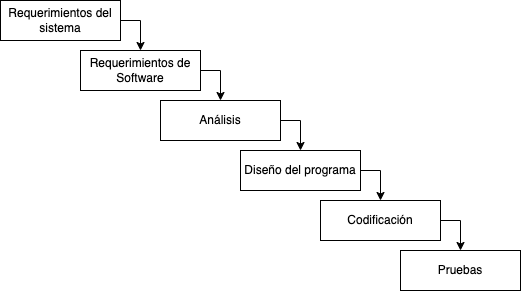
\includegraphics[width=12cm]{img/capitulo_2/cascada2.png}
    \end{center}
    \caption{Modelo Cascada}
    \centering{Fuente: Elaboracion Propia}
    \label{fig:cascada}
\end{figure}

Una vez definida esta secuencia, se creó el concepto de ``Cascada", como un modelo de desarrollo con actividades bien definidas y organizadas con un objetivo independiente dando origen al diseño del primer S.D.M.\footnote{Metodología de Desarrollo de Software} \cite{Bell&Thayer}. En la figura \ref{fig:cascada} la fase de análisis y la de codificación entregan la mayor parte del producto esperado, mientras que las otras fases estan puestas para ser organizadas y planificadas de manera independiente para un mejor manejo de los recursos del proyecto.\\

De acuerdo al modelo Cascada, se enfatiza en la dependecia secuencial del producto entregado en el paso previo. Es decir existe una dependencia que mantiene en espera el diseño del sistema mientras que el análisis del modelo no sea aprobado o concluido y consecuentemente la fase de codificación se verá en espera también hasta que el diseño se concluya.\\

Cada una de las fases guarda una relacion iterativa con el siguiente paso definido en la metodología que asegura la completitud del producto entregado en la fase antetior. Esta relación esta ilustrada en la figura \ref{fig:cascada_iterativa}. Al final de cada etapa, el modelo está diseñado para llevar a cabo una revisión final, que se encarga de determinar si el proyecto está listo para avanzar a la siguiente fase. Este modelo fue el primero en originarse y es la base de todos los demás modelos de ciclo de vida dentro de un proyecto de desarrollo de software.\\

\begin{figure}[H]
    \begin{center}
        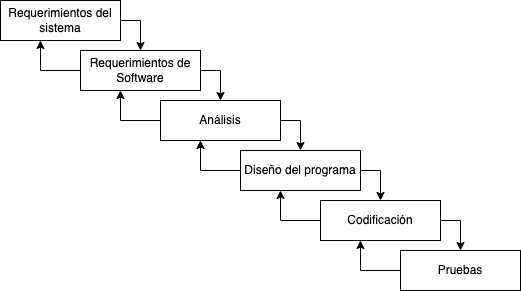
\includegraphics[width=12cm]{img/capitulo_2/cascada_iterativa.png}
    \end{center}
    \caption{Modelo Cascada: Relación iterativa entre las fases sucesivas.}
    \centering{Fuente: Elaboracion Propia}
    \label{fig:cascada_iterativa}
\end{figure}

Existen diferentes versiones de las fases del modelo en cascada y según la versión o enfoque, la cantidad de fases puede variar. Sin embargo las principales son las siguientes:

\begin{enumerate}
    \item Requerimientos del sistema
    \item Requerimientos de Software
    \item Análisis
    \item Diseño del programa
    \item Codificación
    \item Pruebas
    \item Mantenimiento 
\end{enumerate}

A continuacion se detalla cada una de las fases y las actividades que implica cada fase:
